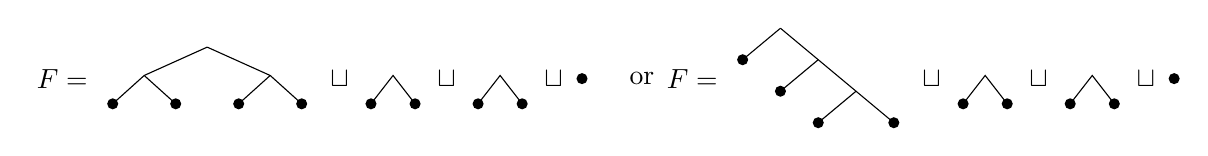
\begin{tikzpicture}[scale=0.8, dot/.style={circle, fill, inner sep=0pt, minimum size=4pt}]
% first workspace: balanced 4-leaf tree, two cherries, one leaf
\node at (-0.8,0.4) {$F=$};
\draw (1.5,0.9) -- (0.5,0.45) -- (0,0); \draw (0.5,0.45) -- (1,0);
\draw (1.5,0.9) -- (2.5,0.45) -- (2,0); \draw (2.5,0.45) -- (3,0);
\foreach \x in {0,1,2,3} \node[dot] at (\x,0) {};
\node at (3.6,0.4) {$\sqcup$};
\draw (4.1,0) -- (4.45,0.45) -- (4.8,0); \node[dot] at (4.1,0) {}; \node[dot] at (4.8,0) {};
\node at (5.3,0.4) {$\sqcup$};
\draw (5.8,0) -- (6.15,0.45) -- (6.5,0); \node[dot] at (5.8,0) {}; \node[dot] at (6.5,0) {};
\node at (7.0,0.4) {$\sqcup$};
\node[dot] at (7.45,0.4) {};
\node at (8.4,0.4) {or};
% second workspace: comb 4-leaf tree, two cherries, one leaf
\begin{scope}[xshift=10cm]
\node at (-0.8,0.4) {$F=$};
\draw (0.6,1.2) -- (0,0.7); \draw (0.6,1.2) -- (2.4,-0.3);
\draw (1.2,0.7) -- (0.6,0.2); \draw (1.8,0.2) -- (1.2,-0.3);
\node[dot] at (0,0.7) {}; \node[dot] at (0.6,0.2) {}; \node[dot] at (1.2,-0.3) {}; \node[dot] at (2.4,-0.3) {};
\node at (3.0,0.4) {$\sqcup$};
\draw (3.5,0) -- (3.85,0.45) -- (4.2,0); \node[dot] at (3.5,0) {}; \node[dot] at (4.2,0) {};
\node at (4.7,0.4) {$\sqcup$};
\draw (5.2,0) -- (5.55,0.45) -- (5.9,0); \node[dot] at (5.2,0) {}; \node[dot] at (5.9,0) {};
\node at (6.4,0.4) {$\sqcup$};
\node[dot] at (6.85,0.4) {};
\end{scope}
\end{tikzpicture}
